\documentclass[12pt]{report}
\usepackage[utf8]{inputenc}
\usepackage{graphicx}
\usepackage{hyperref}
%AMC ajout d'après la doc hyperref overleaf
\hypersetup{
    colorlinks=true,
    linkcolor=blue,
    filecolor=magenta,      
    urlcolor=cyan,
    pdftitle={Pre-study},
    }
\usepackage{todonotes}
\usepackage{tabularray}
%\usepackage{graphicx}
\usepackage{geometry}[top=56mm,bottom=30mm,left=74pt, right=35mm]
\usepackage{parskip}

\usepackage[acronym]{glossaries}
\usepackage[]{glossaries-extra}
\setabbreviationstyle[acronym]{long-short}

\makeglossaries
\glsdisablehyper
\loadglsentries{acronyms}

\begin{document}
\pagenumbering{roman}

\begin{titlepage}
    \begin{center}
        \vspace*{1cm}
            
        \Huge
        \textbf{Multi-Agent System and Digital Twin Models for Security Study of Cyber-Physical System}
        
        \vspace{0.5cm}
        \huge
        Pre-study\\
        \Large
        \textit{October 2022}
            
        \vspace{1.5cm}
    \end{center}
    \LARGE
    %\begin{minipage}{\textwidth}
    \begin{talltblr}[ 
        label = none,
        note{1} = {\large\href{mailto:lagache@kth.com}{lagache@kth.com}},
        note{2} = {\large\href{mailto:oum-el-kheir.aktouf@lcis.grenoble-inp.fr}{oum-el-kheir.aktouf@lcis.grenoble-inp.fr}},
        note{3} = {\large\href{mailto:annabelle.mercier@lcis.grenoble-inp.fr}{annabelle.mercier@lcis.grenoble-inp.fr}},
        ]{}
    Student & Zoé Lagache\TblrNote{1}\\
    KTH Examiner & Roberto Guanciale\\
    KTH Supervisor & Musard Balliu\\
    LCIS supervisor & Oum-El-Kheir Aktouf\TblrNote{2}\\ 
                    & Annabelle Mercier\TblrNote{3}
    \end{talltblr}

    %\end{minipage}
            
    \vfill
    \Large
    Keywords: Multi-Agent System, Digital Twin, Cyber-Physical system, Security
            
\end{titlepage}
\printglossaries

\tableofcontents

\chapter{Introduction}
\pagenumbering{arabic}
\section{Background}
\label{sec:intr:bg}
In a world in an increasing need of control over physical processes, monitoring became mandatory. In order to be accurate enough, more an more systems use electronic systems for monitoring, or even in order to create a digital interface to manipulate physical processes more easily. As an example, cars are for several years now equipped with many sensors to ensure their proper functioning and the safety of the passengers \cite{1435746}. This is what we call \gls{cps}. 


\section{Problem}
\label{sec:intr:pb}
According to the CPS Steering Group \cite{cps_steering_group_cyber-physical_2008}, \gls{cps} are defined as the interaction between physical systems and processes using computations and communication abilities. However, these systems were and are still vulnerable to cyberattacks \cite{wang_security_2010} \cite{singh_review_2020} which could have a huge impact. We can imagine the Cyber-Physical System in an airport monitoring each planes entering or leaving the airport. If such a system undergoes, for instance, a DoS attack, the consequences could be devastating. This is why \gls{cps} need to be protected against cyberattacks. 

\section{Purpose}
\label{sec:intr:purp}
Cyber-Physical Systems can be found in a large range of fields, going from healthcare to the electrical power grid management. Numerous applications of it exist and could benefit from a stronger degree of security.

As an ethical and sustainability perspective, we have to say that this work will discuss attacks on \gls{cps} and may present examples that could be used outside of this work context. However, since the project is primarily concerned with theoretical concepts, this is unlikely. Furthermore, in computer science, simulation is often an energy-intensive process. We will try to tend to optimized solutions but this is not the main goal of this project as we will not focus on a sustainable solution for security of Cyber-Physical systems.

\section{Goals}
\label{sec:intr.goal}
In this master thesis, we propose to study how Multi-Agent System (MAS) and \gls{dt} models can help with this goal and how they complete each other. A Multi-Agent System is a system composed of agents collaborating with each other in order to achieve a common goal. The agents are able to communicate with their local neighbours and, most of the time, only have a local view of the system. MAS are now a trend in the Internet of Things (IoT) field thanks to its decentralization aspect. In the other hand Digital Twins are often associated to a way to track and analyse a system in real time, often in order to predict its behaviour. Both models have the potential to be very useful tools for protecting and preventing cyberattacks on CPS.

\section{Research methodology}
\label{sec:intr:metho}
In order to establish the state of the art, we are going to use mainly Google Scholar and Scopus to look for papers or articles and Zotero to save them. 

The results from the state of the art will lead us to our model creation. Then we will simulate this model with the chosen simulator to check if it works as we want and if we can extract some security claims in relation with the chosen attack model.

From a reproducibility perspective, we will try to provide every sources of paper and tool we use when possible, and will state  when it is not possible, which is unlikely in our case. Indeed, most of the tool we will use should be free. However, some papers may require institutional access or a fee to access the full document.

\section{Delimitations}
\label{sec:intr:delim}
% 


\section{Structure of the thesis}
\label{sec:intr:struct}

\chapter{Background}

In this chapter, we are going to introduce the main areas of the subject by providing the basic background on them. The related work will also be discussed.

\section{Cyber-physical Systems}
\label{sec:bg:cps}
% Don't forget to talk about the question of exploitable surface// the thing that undergoes the damages 
In this section, we are going to explain how \gls{cps} are defined for this thesis and focus on what kind of vulnerability this kind of system is facing an which parameter of the \gls{cia} model is affected for each vulnerability.

\subsection{What are Cyber-physical Systems}
\label{sec:bg:cps:intr}
As indicated in \ref{sec:intr:pb}, \gls{cps} are the combination of the physical world and the cyber space interacting with one another. Most of the time, the cooperation consists in the cyber system monitoring the physical one as seen in Chen~et~al.~\cite{chen_cyber-physical_2022}, Lei~et~al.~\cite{lei_developing_2013} and Tsang~et~al.~\cite{tsang_how_2022} papers. 

\subsection{Cyber-physical System vulnerabilities}
\label{sec:bg:cps:vuln}
\begin{figure}[h!]
    \centering
    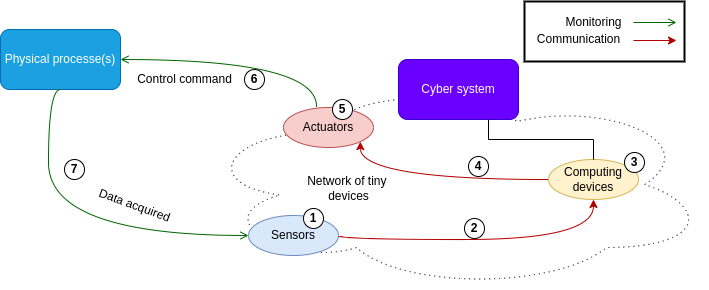
\includegraphics[width = \textwidth]{mind_map_cps_bis.png}
    \caption{\gls{cps} main vulnerabilities}
    \label{fig:cps_vuln}
\end{figure}

In figure \ref{fig:cps_vuln}, we represented a \gls{cps} by two parts: the physical process(es) part and the cyber system. Both of these parts are interacting with each other through sensors and actuators which compose the interface between the two worlds. The cyber system is composed of computing devices receiving data from the sensors, processing it, and sending the result to the actuators.
The green arrows are indicating the monitoring interaction, while the red ones represent the communication within the cyber system.
The numbers point to the parts of the \gls{cps} that are subject to vulnerabilities.

By summarizing the classifications done by Wang~et~al.~\cite{wang_security_2010}, Wazid~et~al.~\cite{wazid_2016} and Singh~et~al.~\cite{singh_review_2020}, we obtained the resulting vulnerabilities mapping:

\subsubsection{Communication attacks}
These attacks have the potential to be operated on all communication links, i. e. at 2, 4, 6 and 7 in figure \ref{fig:cps_vuln}.
Communication attacks can include:

\textit{Eavesdropping:} a passive attack where the attacker is listening to a communication between the two or more nodes of the system. This harms the \textit{confidentiality} of the communication.

\textit{\gls{mitm}:} the base concept is the same as the eavesdropping attack except that the attacker is able to intercept the communication packets and thus to modify them. This attack can impact the \textit{confidentiality} and the \textit{integrity} of the communication.

\subsubsection{Network or routing attacks}
We put in this category the attacks that are the result of a changing of behaviour from one element of the system that can impact changes in the rest of the network. 
All parts of the system from 1 to 5 in figure \ref{fig:cps_vuln} could be impacted by such attacks.

\textit{Blackhole attack:} the attacker is able to corrupt one or several node in the networked system so they advertise their neighboring nodes. This way, they become more attractive in the path-finding algorithm of the nodes. Nevertheless, once the blackhole nodes receive a packet, they drop it. This attack may be called Sinkhole attack in literature while designing Blackhole attacks as several nodes dropping packets, without making themselves more attractive. This attack may perturb the \textit{availability} of some part of the networked system.

\textit{Greyhole attack:} this attack is the same as the Blackhole attack but not all the packets are dropped. A filter is used to select which packets to drop. As well as for the Blackhole attack, the availability is impacted.

\textit{Wormhole attack:} at least two nodes are required to carry out this attack. These nodes are normally not able to communicate with each other but the attacker will upgrade them so they can. This can be done by several ways from simply adding the route in their table to modify the nodes to increase their emission and reception ranges, in the case of they are too far away from each other. This attack does not affect any of the \gls{cia} parameters by itself but it can help multiple follow-up attacks which damage one or several of them.


\subsubsection{Physical attacks}
Physical attacks can be done on the devices that are the closest to the real world, thus on the actuators and on the sensors (1 and 5 in figure \ref{fig:cps_vuln}). 
They can be:

\textit{Side channel attack:} the attacker analyze physical parameters that may vary depending on algorithms implementations and their inputs and is then able to find secret information. This impact the \textit{confidentiality} of the system.

\textit{Fault injection:} the attacker injects a physical fault in the device to change its behaviour in order for it to be malicious. This can be done by injecting quick voltage faults or electromagnetic faults, etc. Such attack have the potential to extract secret information or bypass system security, for example. As well as for the Side Channel Attack, \textit{confidentiality} is compromised here.

\textit{Jamming attack:} the attacker jams the communication hence no packets can be sent and received between the sensor and the signal transforming device. Jamming attacks impact the \textit{availability} of part of the system.

\subsubsection{Application attacks}
\textit{Malware spreading attack:} the attacker spread a piece of malicious code into one or more devices of the system. What the code does vary a lot from revealing secret keys to making a service unavailable, and thus create a \gls{dos}, for example. This kind of attack is mostly observable on the computing devices (3 in figure \ref{fig:cps_vuln}). As a result of its diversity, any of the three parameters of the \gls{cia} model can be harmed.

\subsubsection{Other kind of attacks}
Here are attacks that can be part of several of the previous sections.

\textit{\gls{dos} attack:} the attacker put down a device so it cannot work anymore. This device is often chosen strategically. Ways to achieve this attack are numerous. For example, it can be by sending an extremely high number of messages so a server receiving them is flooded and cannot work properly. If the attack is carried out by several device instead of one, we call that a \gls{ddos} attack. Depending on whether one considers the vulnerable part to be the one that is exploitable or the one that suffers the damage, \gls{dos} is located either on 2 or on 3 in figure \ref{fig:cps_vuln}. It affects the \textit{availability} of the system.


%\subsection{Main attacks}
\subsection{Cyber-physical Systems simulation}
\label{sec:bg:cps:sim}
In computer science, simulation is the act of digitally representing a phenomenon using a model.
It is often used when it is not possible or too expensive to produce the phenomenon in the real world, or when one wants to represent abstract concepts. Simulation is also a way to test our work without having to impact the real world. Critical systems failures can put lives in danger.

The value of \gls{cps} simulation resides in that \gls{cps}s already have information about the real world in a digital environment.
They are studied since several years now and are still confronted to simulation questions as shown by Thule~et~al.~work~\cite{THULE201945}, a 2019 paper presenting a framework for \gls{cps} simulation.

%%% Why do we simulate
%% Good data
% The value of CPS simulation resides in that CPS already have information on the real world in a digital environment allowing us to plug to real data a simulated environment.
% This allows us to have an extremely realistic simulation as it will be based on real world data

%% Important prediction oportunities
% In terms of security, if we are able to simulate environments provided with real data we are also able to predict events on a the specific simulated system. Different models have different results but this gives us a specific possibility to prevent security problems.

%%% How do we simulate 
%% A model 
% As explained in 2.1.3, CPS simulation is based on feeding real data to models of our system. As the problem of recreating an environment perfectly is nearly impossible, research on the topic found different solution allowing, for each model, to solve certain parts of the problem.


\section{Multi-Agent Systems}
\label{sec:bg:mas}
A \gls{mas} is a system with a collection of, at least, two agents, cooperating with each other. These agents are entities containing an algorithm defining their behavior and making them autonomous in their decision making to achieve a common goal. If we add capabilities constraints like computing or memory limitations, then we are talking about embedded agents.
As specified in section \ref{sec:intr.goal}, MAS have been discussed a lot in the computer science field.
It is a model that can be used at different level and in different fields. For example, a \gls{mas} could be a software working on multiple autonomous threads, representing the agents, on a computer. In this case, the separation of the agents is at an application level. Another use case could be a fleet of drones interacting with each other with one drone corresponding to one agent. This diversity of application areas comes from the high customisability and scalability of MAS. 

%\subsection{Multi-Agent System features}
%\subsubsection{Centralization}
%MAS can either be centralized, part centralized or decentralized. 
%A centralized MAS means that information of all the system is gathered in one point. 
%This point can be a central unit or an agent itself that interacts with each agent of the system to collect 
%the wanted information. 

%\subsubsection{Agents}

\subsection{Multi-Agent System and security}
\label{sec:bg:mas:secu}
\gls{mas} are not the first choice for security or safety concerns, due to their autonomy and decentralization that makes them complicated, or even impossible, to monitor. 
However, the approach can solve problems coming from centralization like \gls{spof}. For example, Cai~et~al.~\cite{cai_solutions_2012} propose an Intrusion Detection System based on
an Agents approach where different kind of agents are responsible for monitoring different kind of resources in the system.

Moreover, a subject that is often associated to \gls{mas} is \gls{tms}. 
The \gls{tms} define how an agent can decide to trust another agent or not, depending on specified conditions. It also define the behaviour of the agent in both cases. 

Another interesting addition that can be done is a way to protect the communications between the agents.
This can be done through message signature and encryption.

Building a \gls{mas} integrating a \gls{tms} with secured communications make a system easier to protect in the way that securing one agent is simpler than to monitor an entire system.


\subsection{Multi-Agent System tools}
\label{sec:bg:mas:tool}
This section aims at comparing several tool for simulating \gls{mas}. To gather the tools we are going to talk about, we based our research on previous works done at the LCIS laboratory \cite{bonnet_adrian_securisation_nodate}\cite{derdour_najoua_conception_nodate} in addition to some personal ones as specified in \ref{sec:intr:metho}. Among all these simulators, our first criteria of selection was on the version number. We did not select any tools under version 1.x, in other words that are still at a beta step of development. The second one was on the running platform. We must be able to run the simulator on Debian 11 (Bullseye).

\subsubsection{First selection}
\paragraph{GAMA~\cite{taillandier_building_2019}} is an open source tool for agent based simulation allowing to incorporate agent locations thanks to the GAML language. It was created in 2019.
\paragraph{JACK Intelligent Agents~\cite{busetta_jack_1999}} is a multi-agent system development framework written in Java made in 1999. It has the particularity to use the \gls{bdi} model.
\paragraph{\gls{jade}~\cite{bellifemine_agent_2001}} is also a Java framework for agent-based development but with the difference that JADE is \gls{fipa} compliant. JADE is open source and was developed in 2001.
\paragraph{SARL~\cite{rodrigez_sarl_2014}} is an open source general-purpose agent-oriented programming language that comes with the Janus execution platform\footnote{\href{http://www.sarl.io/runtime/janus/}{http://www.sarl.io/runtime/janus/}}. SARL was developed in 2014.
\paragraph{\gls{madkit}~\cite{gutknecht_madkit_2000}} is an open source library, written in 2000 in Java, for simulating \gls{mas}.
\paragraph{Mesa~\cite{kazil_mesa_2020}} is an open-source agent-based modeling framework. It was written in python and first released in 2021. Mesa comes with a web-browser visualization and aims at offering an easy and customisable way to create agent-based models.
\paragraph{NetLogo}\footnote{\href{https://ccl.northwestern.edu/netlogo/}{https://ccl.northwestern.edu/netlogo/}} is a simulator with the goal to simulate natural or social phenomena. It is continuously improved by the \gls{cclcbm}. NetLogo is open source and comes with its own language and a web-browser interface.
\paragraph{\gls{pade}~\cite{melo_pade_2019}} is another \gls{mas} framework in Python that is \gls{fipa} compliant. It provides an open source tool for developing, executing and managing a \gls{mas}. \gls{pade} was created in 2019 for application on power grids.
\paragraph{\gls{spade}~\cite{gregori_spade_2006}} is a development platform in python using the Jabber communication framework for agents communications. \gls{spade} is also open source and \gls{fipa} compliant. It was developed in 2006.

\subsubsection{The chosen one}
From the pre-selection we made, Mesa stands out. It is one of the most recent work and aims at being easy to use which is needed in our project since we don't have much time to spend to learn new tools. Python is also a language with a big and active community which makes support on this language more accessible. On top of that, the tool was used in previous and current projects done at the laboratory~\cite{bonnet_adrian_securisation_nodate} thus we can get help on how to handle Mesa and the possible difficulties we could encounter.

\section{Digital Twins}
\label{sec:bg:dt}
Digital Twins

\subsection{Digital Twins for security}
\label{sec:bg:dt:sec}
\subsection{Digital Twins simulators}
\label{sec:bg:dt:sim}

%
%
\chapter{References}

\bibliographystyle{IEEEtran}
\bibliography{pre_study.bib}
%\bibliography{references.bib}

\end{document}
